\section{Group Actions}
It is often easier to understand a group if it's doing something, permuting elements, rotating a square etc.

\begin{definition}[Group action]
    Let $G$ be a group and $X$ a non-empty set.
    We say that $G$ \emph{acts} on $X$ if there is a mapping
    \begin{align*}
        \rho : G \times X &\to X \\
        (g, x) &\mapsto \rho(g, x) = g(x)
    \end{align*} 
    such that 
    \begin{enumerate} \addtocounter{enumi}{-1}
        \item if $g \in G$, $x \in X$, then $\rho(g, x) = g(x) \in X$ (implied by notation, but something we should check).
        \item $\rho(gh, x) = \rho(g, \rho(h, x))$. shorthand: $gh(x) = g(h(x))$. \label{action-1}
        \item $\rho(e, x) = x$, shorthand: $e(x) = x$.
    \end{enumerate} 
    When $G$ acts on a set it maps elements of $X$ to $X$ in a way that the multiplication of $G$ is respected.
\end{definition} 

\begin{example} \label{exm:actions} \mbox{}
    \begin{enumerate} \def\labelenumi{\roman{enumi}.} \def\labelenumii{\arabic{enumii}.} 
        \item trivial action $\rho(g, x) = x \; \forall \; x \in X, g \in G$.
        \item $S_n$ acts on $X = \{ 1, 2, \ldots, n \}$ by permuting the elements of $X$.
        e.g. $S_3$ acts on $\{1, 2, 3\}$, $\sigma = \begin{pmatrix}1 & 2\end{pmatrix} \in S_3 : \sigma(1) = 2, \sigma(2) = 1, \sigma(3) = 3$.
        $\tau = \begin{pmatrix}1 & 3\end{pmatrix} \in S_3$, $\tau \sigma = \begin{pmatrix}1 & 3\end{pmatrix} \begin{pmatrix}1 & 2\end{pmatrix} = \begin{pmatrix}1 & 2 & 3\end{pmatrix}$ \\
        $(\tau \sigma)(1) = 2$, $\tau(\sigma(1)) = \tau(2) = 3$. \\
        Similarly subgroups of $S_n$ act on $X$.
        \item $D_8 = \{e, r, r^2, r^3, t, rt, r^2t, r^3t \}$ acts on the edges of a square.
        \begin{figure}
            \centering 
            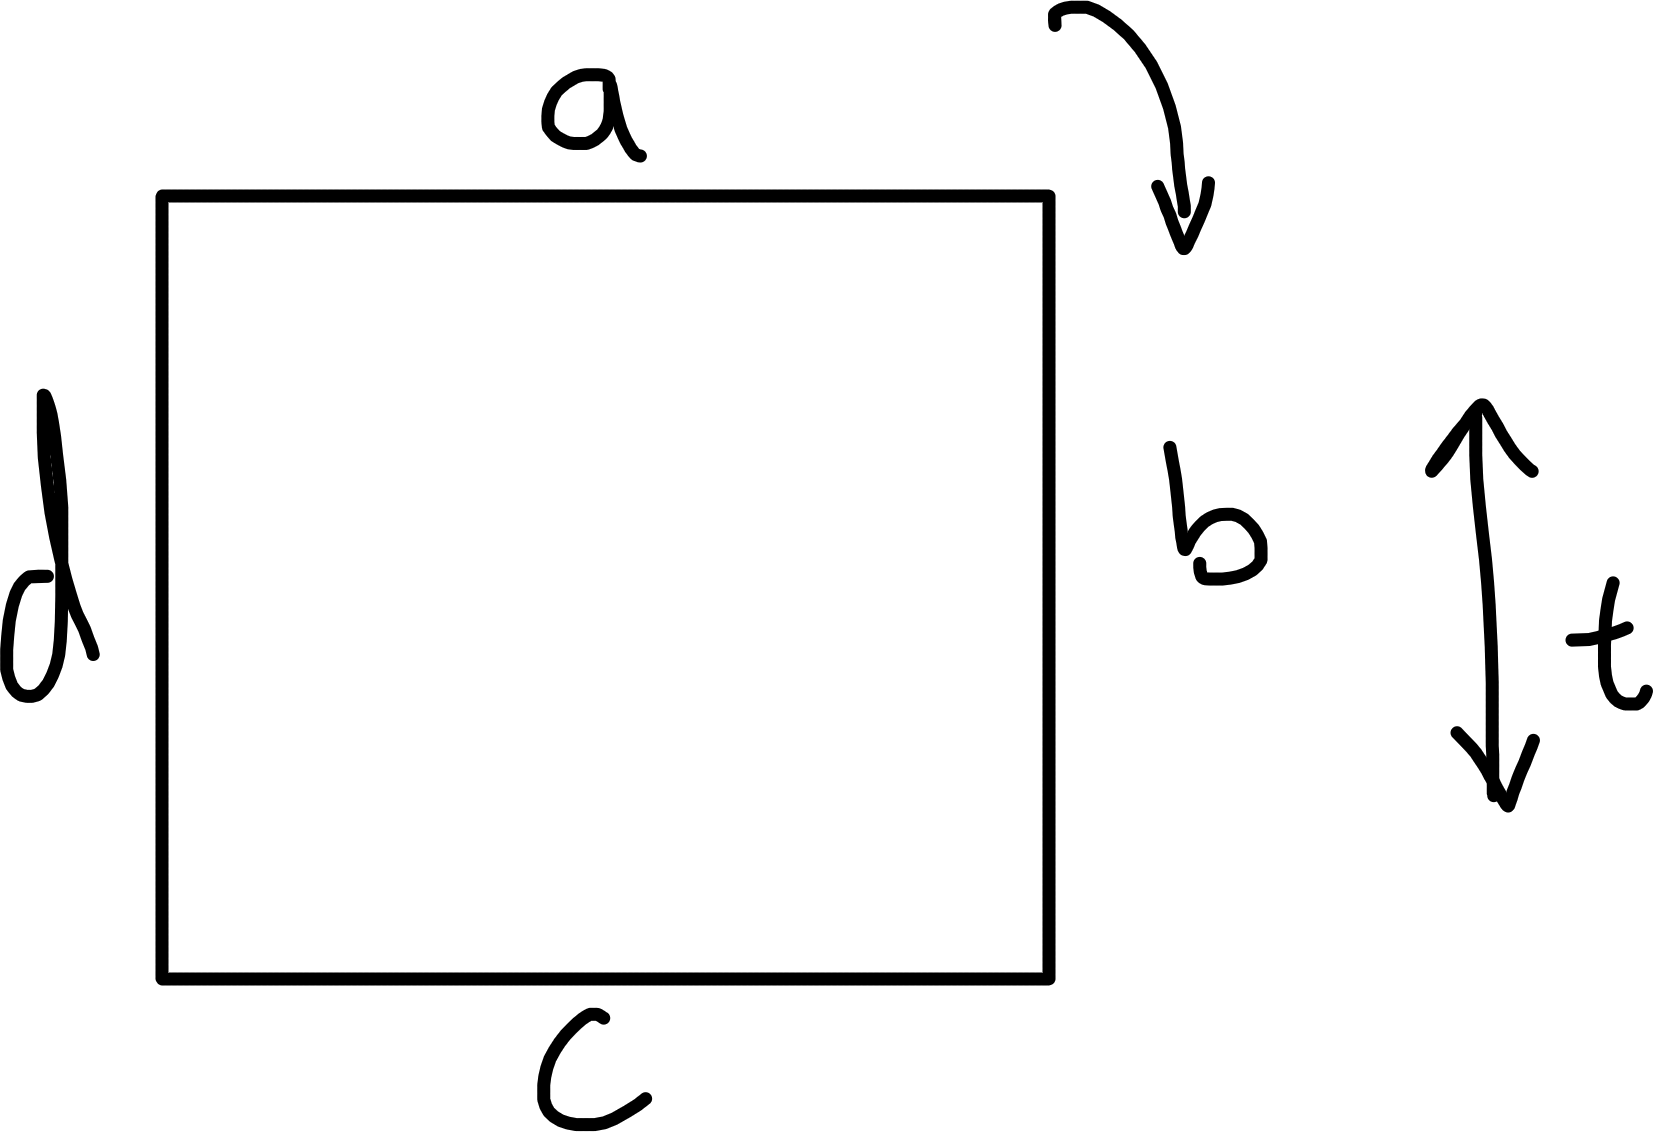
\includegraphics[height=5cm]{figures/06-square-action}
        \end{figure} 
        \begin{align*}
            t(a) &= c & t(c) &= a \\
            t(b) &= b & t(d) &= d. \\
            r(a) &= b.
        \end{align*} 
        Also acts on the vertices of a square.
        \begin{figure}
            \centering 
            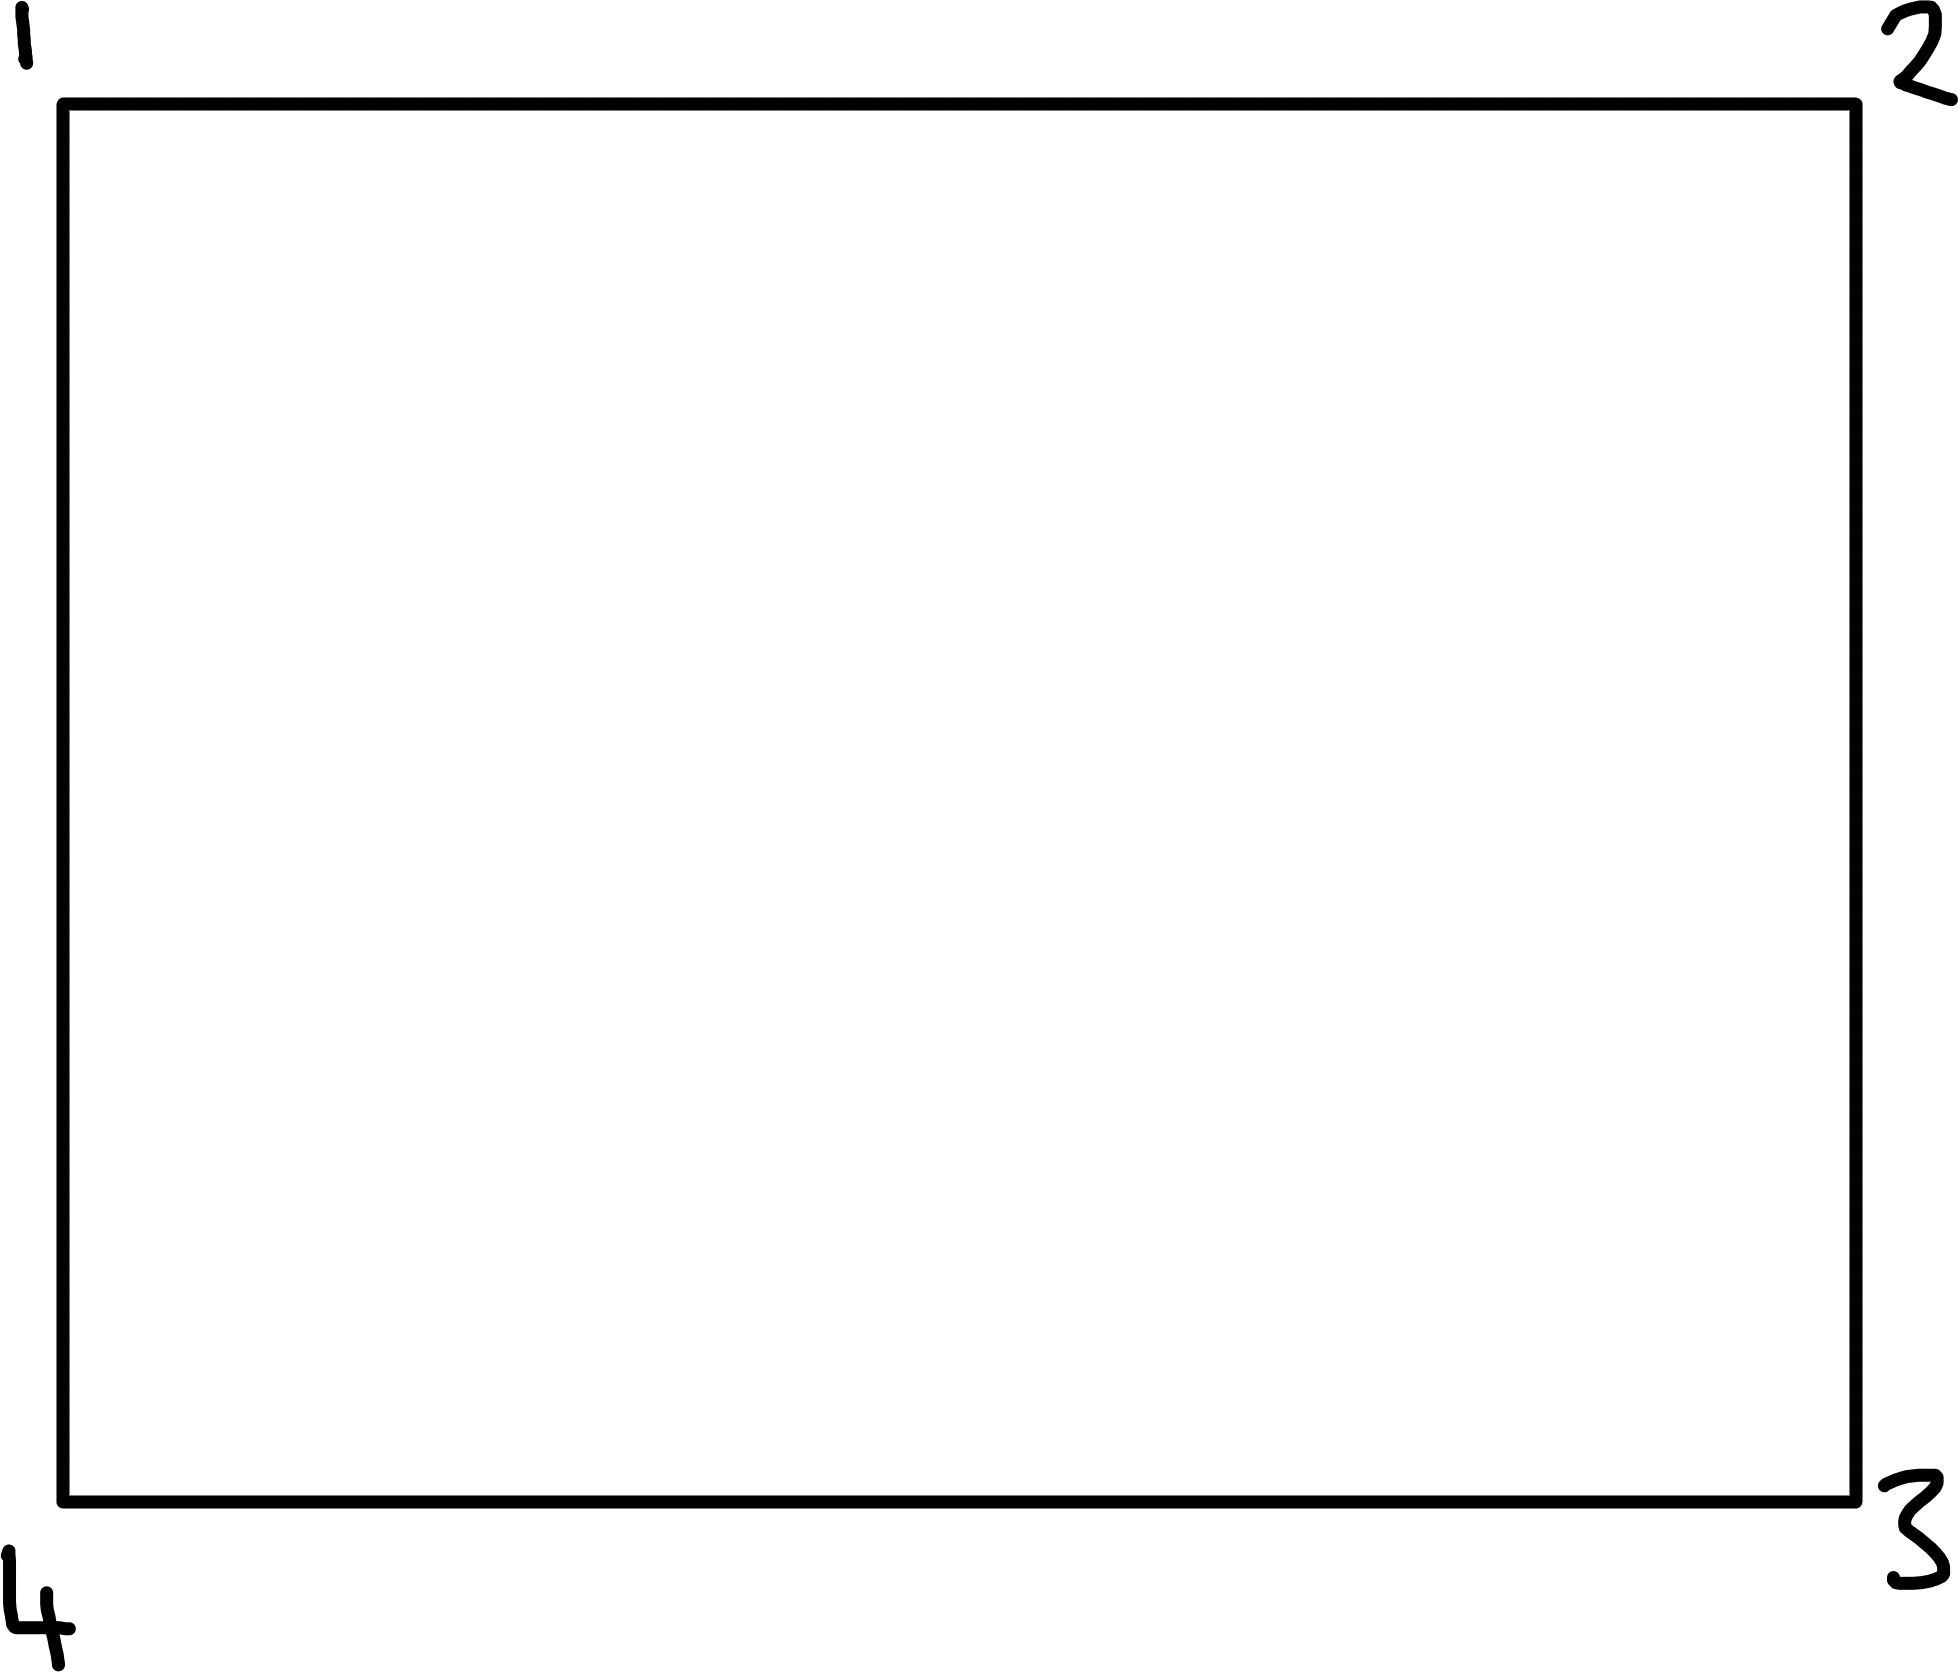
\includegraphics[height=5cm]{figures/06-square-action-vertex}
        \end{figure} 
        \begin{align*}
            t(1) &= 4 & t(4) &= 1 \\
            t(2) &= 3 & t(d) &= 2.
        \end{align*} 
        \item $G$ acts on itself by left multiplication.
        This is called the \emph{left regular action}
        \begin{align*}
            G \times G &\to G \\
            (g, k) &\mapsto gk.
        \end{align*} 
        Check:
        \begin{enumerate} \addtocounter{enumii}{-1}
            \item $gk \in G$ (by closure)
            \item
            \begin{align*}
                \rho(gh, k) &= ghk \\
                \rho(g, \rho(h, k)) &= \rho(g, hk) = ghk \\
                \intertext{Or in shorthand: }
                gh(k) &= ghk \\
                g(h(k)) &= g(hk) = ghk.
            \end{align*} 
            \item $\rho(e, k) = ek = k$.
        \end{enumerate} 
        \item We also have the $G$ \emph{right regular action}
        \begin{align*}
            G \times G &\to G \\
            (g, k) &\mapsto k g^{-1}.
        \end{align*} (we need inverse for \Cref{action-1} to hold.)
        \item $G$ acts on itself by \emph{conjugation}
        \begin{align*}
            G \times G &\to G \\
            (g, k) &\mapsto gkg^{-1}.
        \end{align*} 
        Check: 
        \begin{enumerate} \addtocounter{enumii}{-1}
            \item $gkg^{-1} \in G$ (by closure)
            \item
            \begin{align*}
                \rho(gh, k) &= ghk(gh)^{-1} \\
                &= gh k h^{-1} g^{-1}
                \rho(g, \rho(h, k)) &= \rho(g, hkh^{-1}) = g (h k h^{-1}) g^{-1}
            \end{align*} 
            \item $\rho(e, k) = ek e^{-1} = k$.
        \end{enumerate} 
        \item Let $N \trianglelefteq G$, then $G$ acts on $N$ by conjugation
        \begin{align*}
            G \times N &\to N \\
            (g, n) &\mapsto gng^{-1}.
        \end{align*} 
        0.  $gng^{-1} \in G$ since $N \trianglelefteq G$. \\
        (1) and (2) as above.
        \item Let $H \leq G$, then $G$ acts on the set of left cosets, $(G : H)$, if $H$ in $G$.
        Called the \emph{left coset action}.
        \begin{align*}
            G \times (G : H) &\to (G : H) \\
            (g, kH) &\mapsto gkH.
        \end{align*} 
        \begin{enumerate} \addtocounter{enumii}{-1}
            \item $gkH \in (G : H)$
            \item
            \begin{align*}
                \rho(gh, kH) &= (gh)kH = gh kH. \\
                \rho(g, \rho(h, kH)) &= \rho(g, hkH) \\
                &= g h k H
            \end{align*} 
            \item $\rho(e, kH) = ek H = kH$.
        \end{enumerate} 
    \end{enumerate} 
\end{example} 

\begin{remark}
    Recall a permutation of a set $X$ is a bijection of $X$, \Cref{def:permutation}.
    We have commented that a bijection $f : X \to X$ has a 2-sided inverse, i.e. $\exists \; g : X \to X$ s.t.
    \begin{align*}
        f \circ g (x) &= x \; \forall \; x \in X \\
        g \circ f (x) &= x \; \forall \; x \in X.
    \end{align*}
    Conversely if $f : X \to X$ is a map with a 2-sided inverse then $f$ is a bijection.

    $f \circ g(x) = x \; \forall \; x \in X \implies f$ is surjective, as $f$ is mapping to all elements in $X$ \\
    $g \circ f(x) = x \; \forall \; x \in X \implies f$ is injective, as if $f$ took two elements to the same place then $g$ wouldn't be able to split them up.

    Note 2-sided is necessary:
    \begin{align*}
        \phi : \mathbb{Z} &\to \mathbb{Z} & \psi : \mathbb{Z} &\to \mathbb{Z}\\
        x &\mapsto 2x & 2x & \mapsto x \\
        && 2x + 1 &\mapsto 0 \\
        \phi \psi &= \operatorname{id} &&.
    \end{align*} 
\end{remark} 

\begin{lemma} \label{lem:16}
    Suppose the group $G$ acts on the non-empty set $X$.
    Fix $g \in G$, then the 
    \begin{align*}
        \phi_g : X &\to X \\
        x &\mapsto \rho(g, x) = g(x)
    \end{align*} is a permutation of $X$, i.e. $\phi_g = \operatorname{Sym}(X)$.
\end{lemma} 

\begin{proof}
    Clearly $\phi_g$ is a map from $X$ to $X$.
    We need to show $\phi_g$ is a bijection, enough to show it has a 2-sided inverse.
    %
    \begin{align*}
        \phi_{g^{-1}} \circ \phi_g (x) &= \phi_{g^{-1}} \left( \rho (g, x) \right) \\
        &= \rho(g^{-1}, \rho(g, x)) \\
        &= \rho(g^{-1} g, x) \text{ since $\rho$ is a group action, \ref{action-1}} \\
        &= \rho(e, x) \\
        &= x \; \forall \; x.
    \end{align*} 
    Similarly, $\phi_g \circ \phi_{g^{-1}}(x) = x \; \forall \; x \in X$.
\end{proof} 

\begin{proposition} \label{prp:6}
    Suppose $G$ acts on the set $X$.
    Then the map 
    \begin{align*}
        \Phi : G &\to \operatorname{Sym}(x) \\
        g &\mapsto \phi_g
    \end{align*} as in \Cref{lem:16}, is a homomorphism.
\end{proposition}  

\begin{proof}
    We need to show $\Phi$ is a homomorphism i.e. need
    \begin{align*}
        \Phi(gh) &= \Phi(g) \circ \Phi(h) \\
        \text{i.e. } \phi_{gh} &= \phi_g \circ \phi_h.
    \end{align*}  
    Let $x \in X$
    \begin{align*}
        \phi_{gh}(x) &= \rho(gh, x) \\
        &= \rho(g, \rho(h, x)) \\
        &= \phi_g \circ \phi_h (x).
    \end{align*} 
    This is true $\forall \; x \in X$.
\end{proof} 

\begin{remark} \mbox{}
    \begin{enumerate} \def\labelenumii{\roman{enumii}.} 
        \item \Cref{prp:6} gives us an equivalent definition of a group action.
        If $G$ is a group and $X$ a set such that $\Phi: G \to \operatorname{Sym}(X)$ is a group homomorphism, then 
        \begin{align*}
            \rho : G \times X &\to X \\
            (g, x) &\mapsto \phi_g(x)
        \end{align*} where $\Phi(g) = \phi_g$, is group action.
        \item Using notation of \Cref{prp:6}, by \nameref{thm:six} 
        \begin{align*}
            G / \ker \Phi &\cong \operatorname{Im} \Phi \leq \operatorname{Sym}(X).
            \intertext{Note}
            \ker \Phi &= \{g \in G : \Phi(g) = \text{id}_X \in \operatorname{Sym}(X) \\
            &= \{ g \in G : \phi_g(x) = \rho(g, x) = x \ \forall \; x \in X \} \\
            &\trianglelefteq G \text{ Kernels of homomorphisms are normal subgroups (Sheet 1, q9)}. 
        \end{align*} 
        I.e. all those elements that fix every elements of $X$, that act 'trivially'.

        We say the action is \emph{faithful} if $\ker \Phi = \{ e \}$.

        e.g. the kernels of \Cref{exm:actions}
        \begin{enumerate}
            \item trivial action - $\ker \Phi = G$.
            \item $S_n$ acts on $\{1, \ldots, n\}$ - faithful.
            \item $D_8$ acts on the edges of a square - faithful.
            \item left regular action - faithful.
            \item conjugation - $\ker \Phi = \{g \in G : \underbrace{g k g^{-1} = k}_{gk = kg} \ \forall \; k \in G\} = Z(G)$, the \emph{the centre of} $G$. 'the elements that commute with everything'.
            \item conjugation of $N \trianglelefteq G$. $\ker \Phi = \{ g \in g : g n g^{-1} = n \ \forall \; n \in N\} = C_G(N)$, the \emph{centraliser of $N$ in $G$}.
            \item left coset action -
            \begin{align*}
                \ker \Phi &= \{ g \in G: g kH = kH \ \forall \; k \in G\} \\
                &= \{ g \in G: k^{-1}gk \in H \ \forall \; k \in G\} \\
                &= \{g \in G : g \in k H k^{-1} \ \forall \; k \in G\} \\
                &= \bigcap_{k \in G} k H k^{-1}  \\
                &= \operatorname{Core}_G(H) \trianglelefteq G \\
                \text{and } \underbrace{\operatorname{Core}_G(H)}_\text{core of $H$} &\leq H \text{ (we can set $k = e$)}.
            \end{align*} 
            \emph{Useful Note for exm sheet:} If $\ker \Phi = \{ e \}$, then $G$ is isomorphic to a subgroup of $\operatorname{Sym}(X)$, we write $G \lesssim \operatorname{Sym}(X)$.
            So if $|G| \nmid |\operatorname{Sym}(X)|$ then $\ker \Phi \neq \{e\}$.
        \end{enumerate} 
    \end{enumerate} 
\end{remark} 

\begin{theorem}[Cayley's Theorem] \label{thm:7}
    Any group $G$ is isomorphic to a subgroup of $\operatorname{Sym}(X)$ for some non-empty set $X$.
\end{theorem} 

\begin{proof}
    We take $X$ to be $G$ and consider the left regular action
    \begin{align*}
        G \times G &\to G \\
        (g, h) &\mapsto gh.
    \end{align*} 
    This is a faithful action as $gh = h \; \forall \; h \in G \implies g = e$.
    Thus we have an injective homomorphism 
    \begin{align*}
        \Phi : G &\to \operatorname{Sym}(G)
    \end{align*} and $G \lesssim \operatorname{Sym}(G)$.
\end{proof} 

\begin{definition}[Orbit] \label{def:17}
    Let $G$ act on a set $X$ and $x \in X$.
    The \emph{orbit} of $x \in X$ is given by 
    \begin{align*}
        \operatorname{Orb}_G (x) = \{g(x) : g \in G \} \subseteq X.
    \end{align*} 
    I.e. the set of points in $X$ which $x$ can be mapped to.
\end{definition} 

\begin{example} \mbox{}
    The orbits of \Cref{exm:actions}.
    \begin{enumerate}
        \item trivial action, $\operatorname{Orb}_G (x) = \{ x \}$
        \item $S_n$ acts on $\{1, \ldots, n\}$ - $\operatorname{Orb}_G(1) = X$ (we can get $(1\ a)$ which maps $x$ to any $a$). \\
        If $H = \langle (1\ 2) (3\ 4\ 5) \rangle \leq S_n$ acting on $X = \{ 1, 2, 3, 4, 5\}$ then $\operatorname{Orb}_G(1) = \{1, 2\}$ and $\operatorname{Orb}_G(3) = \{3, 4, 5\}$.
        \item $D_8$ acts on the edges of a square - $\operatorname{Orb}_{D_8}(a) = \{a, b, c, d\}$.
        \item left regular action - $\operatorname{Orb}_G(k) = G$, since $g = g(k^{-1}k) = (gk^{-1})k$ for any $g \in G$.
        \item conjugation - $\operatorname{Orb}_G(k)$
        \begin{align*}
            \operatorname{Orb}_G(k) &= \{g(k) : g \in G\} \\
            &= \{ gkg^{-1} : g \in G \} \\
            &= \operatorname{ccl}_G(k)
        \end{align*}, the \emph{conjugacy class of $k$ in $G$}. If $h \in \operatorname{ccl}_G(k)$ we say $h$ and $k$ are \emph{conjugate}.
    \end{enumerate} 
\end{example} 

\begin{definition}[Transitive orbits] \label{def:18}
    We say $G$ acts \emph{transitively} on $X$ if for any $x \in X$, $\operatorname{Orb}_G(x) = X$.
    Equivalently, if given any pair $x_1, x_2 \in X \; \exists \; g \in G$ s.t. $g(x_1) = x_2$.

    So the left regular action is a transitive action.
\end{definition} 

\begin{lemma} \label{lem:17}
    The distinct $G$-orbits form a partition of $X$
\end{lemma} 

\begin{proof}
    Let $x \in X$, then $x \in \operatorname{Orb}_G(x)$ since $x = ex$. \\
    Suppose $z \in \operatorname{Orb}_G(x) \cap \operatorname{Orb}_G(y)$, we show $\operatorname{Orb}_G(x) = \operatorname{Orb}_G(z) = \operatorname{Orb}_G(y)$. \\
    $z \in \operatorname{Orb}_G(x) \implies \exists \; g \in G$ s.t. $g(x) = z$.
    \begin{align*}
        \text{Suppose } t \in \operatorname{Orb}_G(z) \implies \exists \; h &\in G \text{ s.t. } h(z) = t \\
        \implies t &= h(g(x)) = (hg)(x) \\
        \implies t &\in \operatorname{Orb}_G(x)
        \implies \operatorname{Orb}_G(z) \subseteq \operatorname{Orb}_G(x)
        \text{Similarly } g(x) &= z \\
        x &= e(x) = (g^{-1} g)(x) = g^{-1}(z) \\
        \implies \operatorname{Orb}_G(x) \subseteq \operatorname{Orb}_G(z).
    \end{align*} 
    Thus $\operatorname{Orb}_G(x) = \operatorname{Orb}_G(z)$.
    Similarly, $\operatorname{Orb}_G(z) = \operatorname{Orb}_G(y)$.
\end{proof} 

\begin{remark} \mbox{}
    \begin{enumerate}
        \item We could have proved \Cref{lem:17} by noticing that $x_1 \sim x_2$ if $\exists \; g \in G$ s.t. $g(x_1) = x_2$ is an equivalence relation.
        \item $\operatorname{Orb}_G(x)$ is $G$-invariant, i.e. $g \left( \operatorname{Orb}_G(x) \right) \subseteq \operatorname{Orb}_G(x)$.
        Since if $y \in \operatorname{Orb}_G(x), y = hx$ for some $h \in G \implies g(y) = g(h(x)) = (gh)(x) \in \operatorname{Orb}_G(x)$.
        \item $G$ is transitive on $\operatorname{Orb}_G(x)$.
        \begin{align*}
            \text{Let } y, z &\in \operatorname{Orb}_G(x) \\
            y &= g(x), z = h(x), \text{ for some } g, h \in G. \\
            \text{Then } z &= h(g^{-1}(y)).
        \end{align*} 
    \end{enumerate} 
\end{remark} 

\begin{definition}[Stabiliser] \label{def:19}
    Let $G$ act on $X$ and $x \in X$.
    The \emph{stabiliser} of $x$ in $G$ is given by
    \begin{align*}
        \operatorname{Stab}_G(x) &= \{ g \in G : g(x) = x \} \\
        &\subseteq G.
    \end{align*} 
    i.e. all those elements in $G$ that fix $x$.
\end{definition} 

\begin{example} \mbox{}
    The stabilisers of \Cref{exm:actions}.
    \begin{enumerate}
        \item trivial action - $\operatorname{Stab}_G(x) = G$.
        \item $S_n$ on $X = \{1, 2, \ldots, n\}$ - $\operatorname{Stab}_G(1) \cong S_{n-1}$.
        \item $H = \langle \begin{pmatrix}1 & 2\end{pmatrix} \begin{pmatrix}3 & 4 & 5\end{pmatrix} \rangle$ on $X$ - $\operatorname{Stab}_H(1) = \langle \begin{pmatrix}3 & 4 & 5\end{pmatrix} \rangle$.
        \item $D_8$ - $\operatorname{Stab}_{D_8}(b) = \{e, t\}$. \\
        \item left regular action - $\operatorname{Stab}_G(k) = \{e\}$, $gk = k \implies g = e$.
        \item conjugation - \begin{align*}
            \operatorname{Stab}_G(k) &= \{g \in G : g(k) = k\} \\
            &= \{g \in G : g k g^{-1} = k\} \\
            &= \{g \in G : g k = kg \} \\
            &= C_G(k), \emph{ centraliser of $k$ in $G$}.
        \end{align*} I.e. all those elements of $G$ that commute with $k$.
    \end{enumerate} 
\end{example} 

\begin{lemma} \label{lem:18}
    $\operatorname{Stab}_G(x)$ is a subgroup of $G$.
\end{lemma} 

\begin{proof} \mbox{}
    \begin{itemize} 
        \item $e(x) = x \implies e \in \operatorname{Stab}_G(x)$.
        \item \begin{align*}
            \text{if } g, h &\in \operatorname{Stab}_G(x) \\
            (gh)(x) &= g(h(x)) \\
            &= g(x) \\
            &= x \implies gh \in \operatorname{Stab}_G(x).
            \end{align*} 
        \item \begin{align*}
            g &\in \operatorname{Stab}_G(x) \\
            g(x) &= x \\
            x &= e(x) = (g^{-1} g)(x) = g^{-1}(gx) \\
            &= g^{-1}(x) \\
            \implies g^{-1} &\in \operatorname{Stab}_G(x).
        \end{align*} 
        \item Associativity is inherited from $G$.
    \end{itemize} 
\end{proof} 

\begin{remark} 
    Recall, \Cref{prp:6} \begin{align*}
        \Phi : G &\to \operatorname{Sym}(X) \\
        \ker \Phi &= \{ g \in G : g(x) = x \; \forall \; x \in X \} \\
        &= \bigcap \operatorname{Stab}_G(x).
    \end{align*}
\end{remark} 

\begin{theorem}[Orbit-Stabiliser Theorem]
    Let $G$ be a finite group acting on a non-empty set $X$.
    Then $\operatorname{Stab}_G(x) \leq G$ and 
    \begin{align*}
        |G| = |\operatorname{Stab}_G(x)| |\operatorname{Orb}_G(x)|.
    \end{align*} 
\end{theorem} 

\begin{remark}
    We actually prove that $|G : \operatorname{Stab}_G(x)|$, the number of left cosets of $\operatorname{Stab}_G(x)$ in $G$, is equal to $|\operatorname{Orb}_G(x)|$, a more general statement.
\end{remark} 

\begin{proof}
    $(G : \operatorname{Stab}_G(x))$ is the set of left cosets of $\operatorname{Stab}_G(x)$ in $G$.
    Consider the map 
    \begin{align*}
        \theta : \operatorname{Orb}_G(x) &\to (G : \operatorname{Stab}_G(x)) \\
        g(x) &\mapsto g \operatorname{Stab}_G(x).
    \end{align*}  
    $\theta$ is well-defined: 
    \begin{align*}
        g(x) = h(x) \implies h^{-1}g(x) (x) &= x \\
        \implies h^{-1}g &\in \operatorname{Stab}_G(x) \\
        \implies g \operatorname{Stab}_G(x) &= h \operatorname{Stab}_G(x) \text{ by \Cref{lem:eleven}} \\
        \implies \theta(g(x)) &= \theta(h(x)).
    \end{align*} 
    $\theta$ is injective: 
    \begin{align*}
        \theta(g(x)) &= \theta(h(x)) \\
        \implies g \operatorname{Stab}_G(x) &= h \operatorname{Stab}_G(x) \\
        \implies h^{-1}g &\in \operatorname{Stab}_G(x) \text{ by \Cref{lem:eleven}} \\
        \implies h^{-1}g(x) &= x \\
        \implies g(x) &= h(x).
    \end{align*}
    $\theta$ is surjective:
    \begin{align*}
        \text{Given } g \operatorname{Stab}_G(x) &\in (G : \operatorname{Stab}_G(x)) \\
        \text{then } g(x) &\in \operatorname{Orb}_G(x) \\
        \text{ and } \theta(g(x)) &= g \operatorname{Stab}_G(x).
    \end{align*} 
    Thus $\theta$ is a well-defined bijection.
\end{proof} 